\documentclass[a4paper,10pt]{article}

\usepackage{subfig}
\usepackage{float}
\usepackage{graphicx}
\usepackage{verbatim}
\usepackage{amsthm}
\usepackage{amsmath}
\usepackage{amssymb}
\usepackage{geometry}

\newtheorem{defn}{Definition}
\newtheorem{prop}{Proposition}
\newtheorem{theorem}{Theorem}
\newtheorem{cor}{Corollary}

%opening
\title{Opinion-dependent Rewiring Model}
\author{Sam Magura, Vitchyr Pong}

\begin{document}

\maketitle
\section{Model Definition}
The process operates on a graph $G = (V, E)$. Each vertex $v = \langle v_1, v_2, \ldots, v_D \rangle$ where $v_1$, $v_2$, and so on represent the opinions of $v$. Initially, each vertex is placed randomly in the \emph{opinion space} $\Omega = [0, 1]^D$. The distance function $d(x, y)$ gives the \emph{opinion distance} between two vertices $x$ and $y$. We use
\begin{equation}
 d(x, y) = |x_1 - y_1| + |x_2 - y_2| + \ldots.
\end{equation}
Let the constant $p = 1 / D$ so that $p \; d(x, y) \leq 1$ for any possible $\{x, y\}$.  
\\\\Each iteration, do the following.
\begin{enumerate}
 \item Randomly choose an edge from the graph.
 \item Apply a random orientation $(x, y)$ to the edge.
 \item \label{item:z} Randomly choose a vertex $z$ from the set of all vertices that are neither $x$ nor adjacent to $x$.
 \item With probability
 \begin{equation}
 \label{exp:pr}
  p \; d(x, y) \; \min\left(1, \frac{d(x, y)}{d(x, z)}\right), 
 \end{equation}
remove the edge $\{x, y\}$ and add the edge $\{x, z\}$. 
\end{enumerate}
In Expression \ref{exp:pr}, $p \; d(x, y)$ represents the chance that $\{x, y\}$ is marked for removal and $\min(1, \frac{d(x, y)}{d(x, z)})$ represents the chance that the addition of $\{x, z\}$ is accepted. We say ``$\{x, y\}$ is marked for removal'' since the edge is only removed if the addition of $\{x, z\}$ is also accepted. Thus, the greater the opinion distance of the original edge $\{x, y\}$, the greater the chance that that edge is marked for removal. The addition of the new edge $\{x, z\}$ is always accepted if the new distance is less than the original distance. However, if the new distance is greater, the addition is accepted with probability $d(x, y) / d(x, z).$

In many network models, multiple edges are allowed because they are relatively unlikely in large networks. However, if multiedges are allowed in this model, many edges will accumulate between pairs of vertices that have especially low opinion distances. Because of this, we prevent the creation of multiedges by refusing to select a $z$ that is already to adjacent to $x$ in Step \ref{item:z}.

\section{Stationary Distribution}
The model is a Markov Chain because the probability of transitioning from a state $G$ to a state $H$ is dependent only $G$ and $H$. 

\begin{defn}
 Graphs $G = (V, E_G)$ and $H = (V, E_H)$ are the same state in the Markov Chain if and only if $E_G = E_H$.
\end{defn}


\paragraph{Transition probability} Consider states $G$ and $H$ such that $\{x, y\}$ is in $G$ but not $H$, and $\{x, z\}$ is in $H$ but not $G$. For a transition from $G$ to $H$, the following must occur.
\begin{enumerate}
 \item The edge $\{x, y\}$ is selected. This occurs with probability $\frac{1}{m}$.
 \item The orientation $(x, y)$ is chosen. This occurs with probability $\frac{1}{2}$.
 \item Vertex $z$ is selected in Step \ref{item:z} of the model definition. This occurs with probability $\frac{1}{m - k(x) - 1}$ where $k(x)$ gives the degree of $x$, since $z$ is selected randomly from the set of all vertices that are neither $x$ nor adjacent to $x$.
 \item The rewiring is accepted. This occurs with probability $ p \; d(x, y) \; \min(1, \frac{d(x, y)}{d(x, z)}).$
\end{enumerate}
Therefore the transition probability is 

\begin{equation}
\label{eqn:pgh}
 P(G, H) = \frac{ p \; d(x, y) \; \min\left(1, \frac{d(x, y)}{d(x, z)}\right)}{2m \left(m - k(x) - 1\right)}.
\end{equation}

\begin{theorem}
  The detailed balance condition is satisfied by the stationary distribution
\begin{equation}
 \pi(G) = b \prod_{e} \frac{1}{d(e)^2}
\end{equation}
where $b$ is some normalization coefficient, $e$ is any edge in graph $G$, and $d(e)$ gives the distance between the endpoints of edge $e$.
\end{theorem}
\begin{proof}
 The detailed balance condition is
 \begin{equation}
 \pi(G) \: P(G, H) = \pi(H) \: P(H, G).
\end{equation}
Without loss of generality, suppose $d(x, y)$ is greater than $d(x, z)$. Substituting in the transition probabilities from Equation \ref{eqn:pgh} and the proposed stationary distribution $\pi$, we have

\begin{equation}
\frac{ p \; d(x, y)}{2m \left(m - k(x) - 1\right)}
\left(b\prod_{e \in E_G} \frac{1}{d(e)^2}\right) =
\frac{ p \; d(x, z)^2}{2m \; d(x, y) \left(m - k(x) - 1\right)}\:
\left(b\prod_{e \in E_H} \frac{1}{d(e)^2}\right).
\end{equation}
This simplifies to
\begin{equation}
d(x, y)^2 \prod_{e \in E_G} \frac{1}{d(e)^2} =
d(x, z)^2 \prod_{e \in E_H} \frac{1}{d(e)^2}
\end{equation}
since the degree of $x$ does not change. Because the only difference between $G$ and $H$ is that $G$ has an edge $\{x, y\}$ that $H$ does not and $H$ has an edge $\{x, z\}$ that $G$ does not, the detailed balance condition holds for the proposed stationary distribution $\pi$.
\end{proof}

\section{Constructive Model}
\begin{theorem}
\label{thm:perc}
When the rewiring model has reached the steady state, the probability that an edge $e^*$ is present is approximately
\begin{equation*}
 \frac{c}{d(e^*)^2 + 1} \mbox{\;\;\;with\;\;\; } c =\frac{m}{\sum\limits_{e \in K_n} \frac{1}{d(e)^2 + 1}}
\end{equation*}
where $n = |V|$, $m = |E|$, and $K_n$ is the complete graph on $n$ vertices.
\end{theorem}
\begin{proof}
For a constructive model in which each edge $e$ is independently present with probability $P(e)$, the probability that a particular graph $G$ is produced is
\begin{equation}
 \mu(G) = \prod\limits_{e \in G} \frac{P(e)}{1 - P(e)} \prod\limits_{e \in K_n} (1 - P(e)).
\end{equation}
We want to find the function $P(e)$ such that $\mu(G)$ is approximately equal to $\pi(G)$. Because the expressions for $\mu(G)$ and $\pi(G)$ both contain a product over all edges $e \in G$ multiplied by some factor which is independent of $G$, we can write
\begin{equation}
\label{eqn:proportional}
 \frac{P(e)}{1-P(e)} \propto \frac{1}{d(e)^2} \;\;\;\;\longrightarrow\;\;\;\; P(e) = \frac{c}{d(e)^2 + 1}.
\end{equation}
Since each state in the rewiring model contains exactly $m$ edges, the expected the number of edges of a graph produced by the constructive model should be $m$:
\begin{equation}
\label{eqn:sum-to-m}
 \sum_{e \in K_n} P(e) = m.
\end{equation}
By substituting Equation \ref{eqn:proportional} into Equation \ref{eqn:sum-to-m}, we reach an expression for the coefficient $c$:
\begin{equation}
\label{eqn:c}
 c = \frac{m}{\sum\limits_{e \in K_n} \frac{1}{d(e)^2 + 1}}.
\end{equation}
\end{proof}

\begin{theorem}
\label{thm:c}
For large $n$,
 \begin{equation}
  c = \frac{2\, m}{n^2} \; \left[\,\int\limits_\Omega \int\limits_\Omega \frac{du\, dv}{d(u, v)^2 + 1}\right]^{-1}
 \end{equation}
where $\Omega$ is the opinion space $[0, 1]^D$.
\end{theorem}
\begin{proof}
 The sum in the denominator of our expression for $c$ (Equation \ref{eqn:c}) can be rewritten as
 \begin{equation}
 \label{eqn:double-sum}
  \frac{1}{2} \sum\limits_{u}\sum\limits_{v \neq u} \frac{1}{d(u, v)^2 + 1}
 \end{equation}
 where $u$ and $v$ are any vertices in the graph. For large $n$, vertices are evenly distrbuted within the opinion space since they are placed randomly. Therefore, there are $n \,du$ vertices in an interval $du$ with dimensions $du_1, du_2, \ldots, du_D$, and $\frac{1}{2}(n\, du)(n\, dv)$ edges between vertices in $du$ and vertices in $dv$. Because the sums in Expression \ref{eqn:double-sum} are computed over $n$ and $n - 1$ vertices respectively, and $n$ is large, we can express the two sums as a double integral:
 \begin{equation}
  \frac{1}{2}\, n^2 \int\limits_\Omega \int\limits_\Omega \frac{du \, dv}{d(u, v)^2 + 1}.
 \end{equation}
\end{proof}
\begin{prop}
 For $D=1$ and large $n$,
 \begin{equation*}
  c = \frac{4 \,m}{n^2 \,(\pi - \ln 4)}.
 \end{equation*}
\end{prop}
\begin{proof}
For $D=1$, the double integral in Theorem \ref{thm:c} reduces to
 \begin{equation}
  \frac{1}{2}\, n^2 \int\limits_0^1 \int\limits_0^1 \frac{du_1 \, dv_1}{(u_1 - v_1)^2 + 1}.
 \end{equation}
We evaluate this integral to reach our result.
\end{proof}

\section{Expected Degree}
\begin{theorem}
\label{thm:lambdax}
The expected degree of a vertex $x$ is
 \begin{equation}
 \lambda(x) = c\,n\int\limits_\Omega \frac{du}{d(x, u)^2 + 1}.
\end{equation}
\end{theorem}
\begin{proof}
The expected number of vertices in an interval $I$ with dimensions $du_1, du_2, \ldots, du_D$  is $n \cdot du_1 \cdot du_2 \cdots du_D$ because $n$ vertices are evenly distrbuted within $\Omega$. From Theorem \ref{thm:perc}, we see that expected number of edges $\{x, u\}$ where $u \in I$ is $\frac{c}{d(x, u)^2 + 1} \, n \, du$. Thus the expected degree of $x$ is this function integrated over $\Omega$.
\end{proof}

\begin{prop}
For $D = 1$, The expected degree of a vertex $x = x_1$ is
 \begin{equation}
 \lambda(x) = c\,n\left(\tan^{-1} x + \tan^{-1} (1-x)\,\right).
\end{equation}
\end{prop}
\begin{proof}
When $D=1$, Theorem \ref{thm:lambdax} reduces to
\begin{equation}
 \lambda(x) = c\,n\;\int\limits_{0}^{1} \frac{du}{(x - u)^2 + 1}.
\end{equation}
Evaluating the integral yields our result.
\end{proof}

\begin{figure}
 \centering
 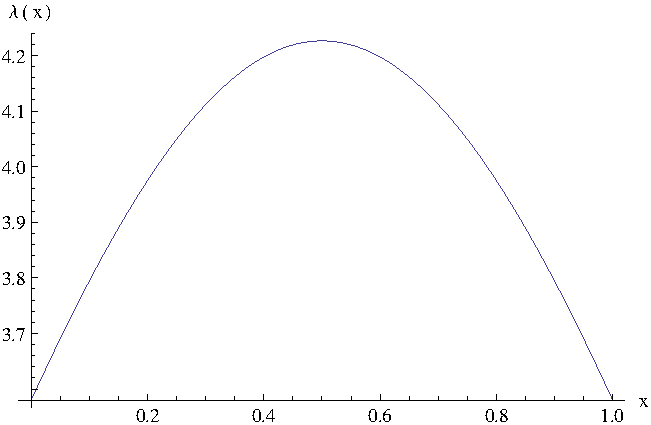
\includegraphics{images/lambdaofx.pdf}
 \caption{A plot of expected degree $\lambda(x)$ vs. opinion $x$ when the mean degree is 4. The curve has reflectional symmetry across $x = \frac{1}{2}$ as expected.}
 \label{fig:lambdaofx}
\end{figure}


\begin{prop}
\label{prop:R1}
 For $D=1$, $\lambda(x) \in R_1 = [c\,n\,\frac{\pi}{4},\; 2\,c\,n \tan^{-1}\frac{1}{2}]$ for any $x$.
 \end{prop}
\begin{proof}
First we determine the critical values of $\lambda(x)$ with $x \in [0, 1]$. The derivative is
\begin{equation}
 \frac{d\lambda}{dx} = c\,n\left(\frac{1}{1+x^2} - \frac{1}{1+(1-x)^2} \right).
\end{equation}
Thus $\frac{d\lambda}{dx} = 0$ if and only if $x^2 = (1 - x)^2$, and $x=\frac{1}{2}$ is the one critical value. From Figure \ref{fig:lambdaofx}, we see that $\lambda(\frac{1}{2}) = 2\,c\,n \tan^{-1}\frac{1}{2}$ is the maximum expected degree. From the figure, it is also clear that the minima of $\lambda(x)$ lie at the endpoints of the interval. The minimum expected degree is $\lambda(0) = \lambda(1) = c\,n\,\frac{\pi}{4}.$
\end{proof}

\begin{prop}
 For $D=1$, the distribution of expected degrees is given by
 \begin{equation}
  M(\lambda) = n \,\frac{dx}{d\lambda}
 \end{equation}
when $\lambda \in [c\,n\,\frac{\pi}{4},\; 2\,c\,n \tan^{-1}\frac{1}{2}]$ and $M(\lambda) = 0$ otherwise. \end{prop}
\begin{proof}
$M(\lambda)$ is obviously 0 when $k$ is not in the range of possible expected degrees, $R_1$. Let $x(\lambda)$ give the opinion of a vertex with expected degree $\lambda$ and always return a value in $[0, 1/2]$. With $\Delta \lambda \to 0$, all vertices in the interval $[x(\lambda), x(\lambda + \Delta \lambda)]$ have expected degree $\lambda$. Because vertices are spread evenly within the opinion space, the number of vertices that have degree $\lambda$ is proportional to $x(\lambda + \Delta \lambda) - x(\lambda)$. Therefore
\begin{equation}
 M(\lambda) = a \lim\limits_{\Delta \lambda \to 0} \frac{x(\lambda + \Delta \lambda) - x(\lambda)}{\Delta \lambda} = a \, \frac{dx}{d\lambda}
\end{equation}
for constant $a$. However, recall from the proof for Proposition \ref{prop:R1} that $\frac{d\lambda}{dx} = 0$ at the maximum of $\lambda(x)$ at $x=1/2$. Thus $M(\lambda) = a \, \frac{dx}{d\lambda}$ only when $\lambda \in  [c\,n\,\frac{\pi}{4},\; 2\,c\,n \tan^{-1}\frac{1}{2})$. Because the number of real numbers in $[0, 1]$ is infinite, the probability that a vertex $x$ is exactly $1/2$ is 0; thus $M(2\,c\,n \tan^{-1}\frac{1}{2}) = 0$. To determine $a$, we note that the relationship 
\begin{equation}
\label{eqn:Msum}
 \int\limits_{0}^\infty M(\lambda)\, d\lambda = n
\end{equation}
must hold. Substituting $a \, \frac{dx}{d\lambda}$ for $M(\lambda)$ gives us 
\begin{equation}
 a\int\limits_{0}^\infty \frac{dx}{d\lambda} \, d\lambda = a\int\limits_{0}^1 dx = a.
\end{equation}
Thus $a = n$.
\end{proof}
\end{document}
